\documentclass[11]{article}

\usepackage[inline]{enumitem}
\usepackage{graphicx}
\usepackage{gensymb}
\usepackage{float}

\usepackage[numbered,framed]{matlab-prettifier}
\let\ph\mlplaceholder % shorter macro
\lstMakeShortInline"

\lstset{
  style              = Matlab-editor,
  basicstyle         = \mlttfamily,
  escapechar         = ",
  mlshowsectionrules = true,
}

\title{
  Hand Written
  Digit Recognition
  }
  
\date{}
\author{STUDENT ID: 1057404 }

\hyphenation{thatshouldnot}

\begin{document}
\maketitle 	

\section{Introduction}
This project designs and implements a neural network to optically recognise hand written digits. Starting with the fewest number of layers and increasing subsequently, the network generalisation is optimised through adjusting parameters of learning rate, batch size, epoch count, data preprocessing and weight decay rate.

The data set used contains records from 43 participants and is split between a training set and a test set. The training set of 3823 records was collected from 30 of the participants. The test set of 1797 records was collected from the remaining 13. Each record contains 64 pixels of an 8x8 image (e.g. \ref{fig:digits} followed by the digit it represents. The pixel intensity is between 0 and 16. 

\begin{figure}[h]
\centering
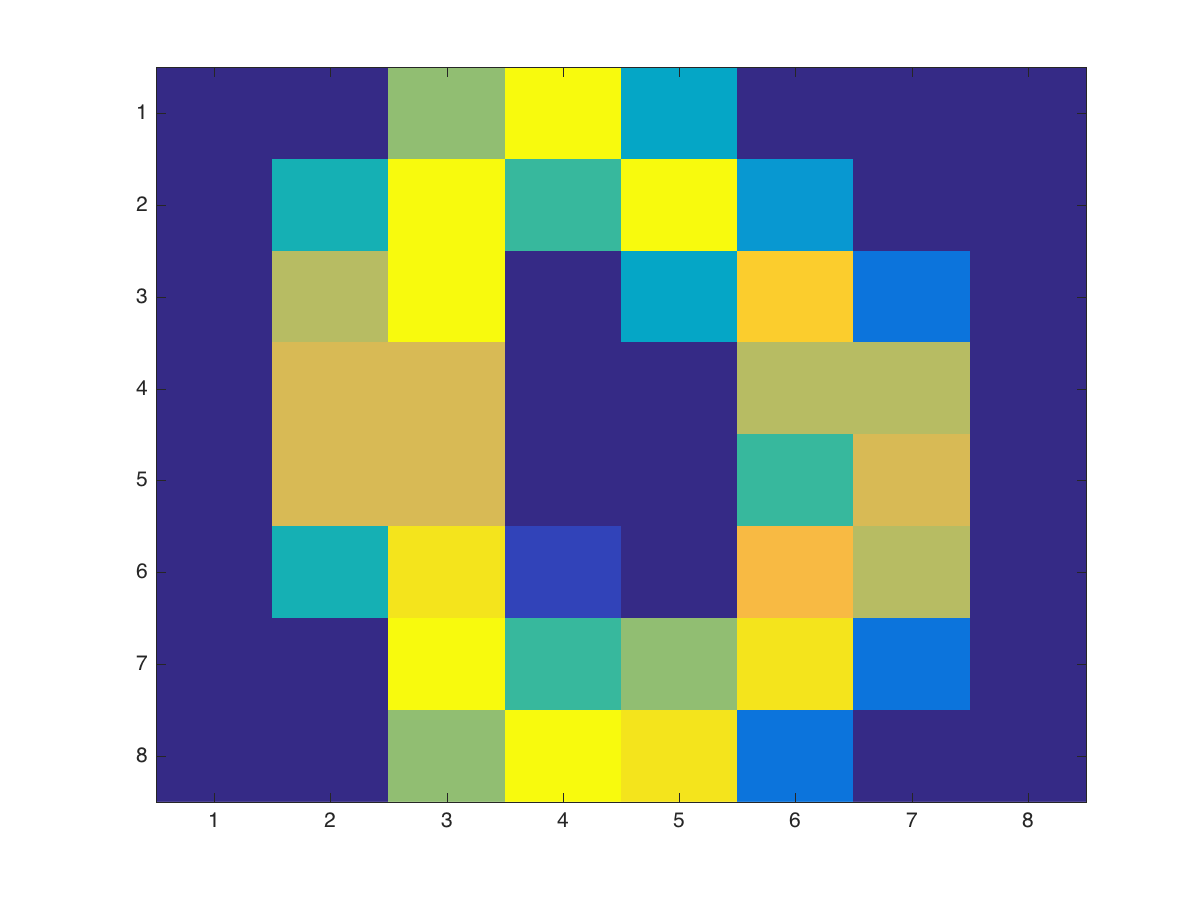
\includegraphics[width=0.4\textwidth]{zero.png}
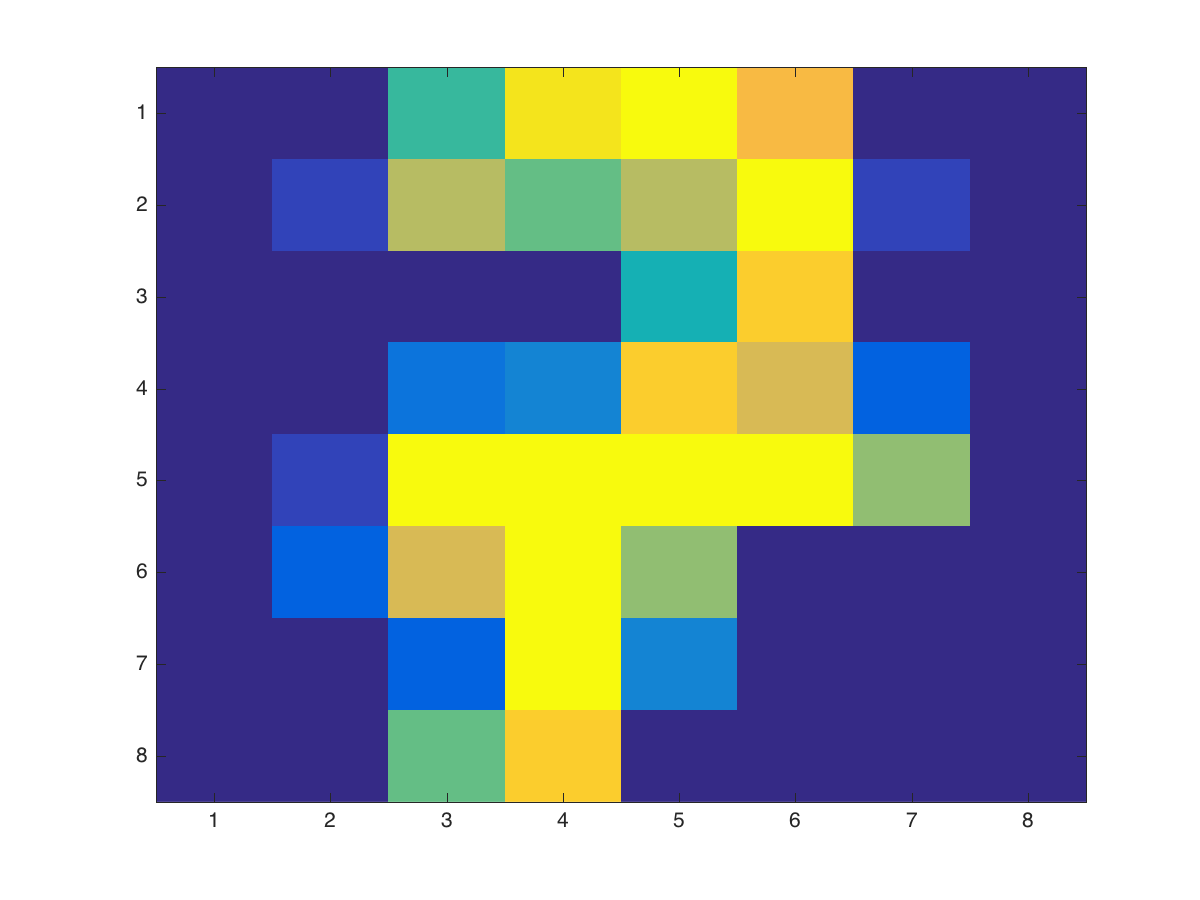
\includegraphics[width=0.4\textwidth]{seven.png}
\caption{Example images from training set}
\label{fig:digits}
\end{figure}
\section{Design}

The resulting design is a two layer perceptron neural network using the cross entropy cost function. This cost function was selected as the problem is one of classification rather than regression (i.e. each feature set belongs to a digit class).

When using cross entropy, the activation function generally used is a sigmoid. As its output ranges from 0 to 1, the activation of a neuron is analogous to a probability function. Whilst sigmoid is used for hidden layer activations, softmax is used for the output layer. This ensures that the sum of probability for each class activation does not exceed 1. 

The network's input is 69 features. The fist 64 represent the image pixels with an additional 5 features extracted from pixel covariance and mean location.  The hidden layer size is 60 nodes and the output layer is 10 nodes ( one for each activation class ). 

Additional training records were created by rotating each feature set to a varying range between -20 and +20 degrees clockwise (fig. \ref{fig:rotated}. The process aids detection for digits that are not properly aligned. The additional features of covariance and mean pixel location serves the same purpose. 
\begin{figure}[h]
\centering
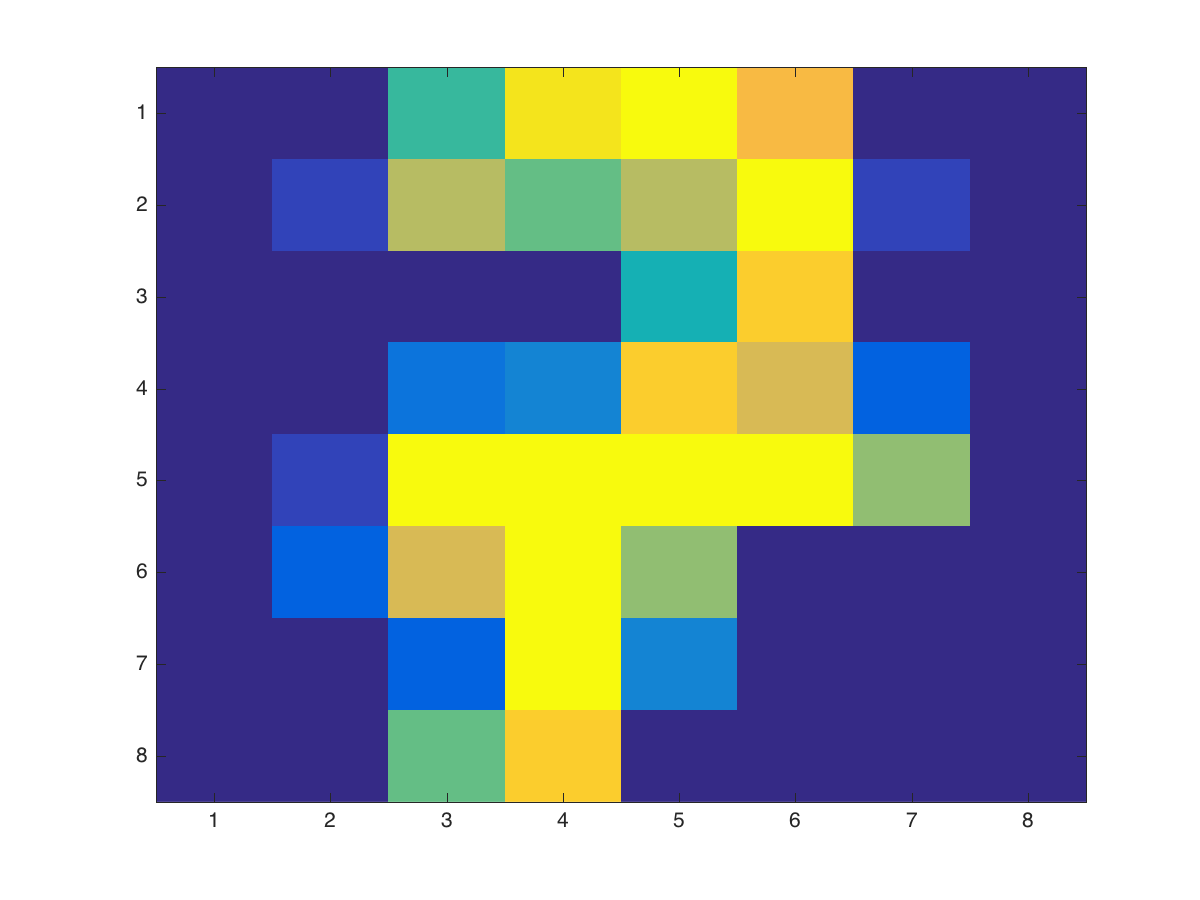
\includegraphics[width=0.4\textwidth]{seven.png}
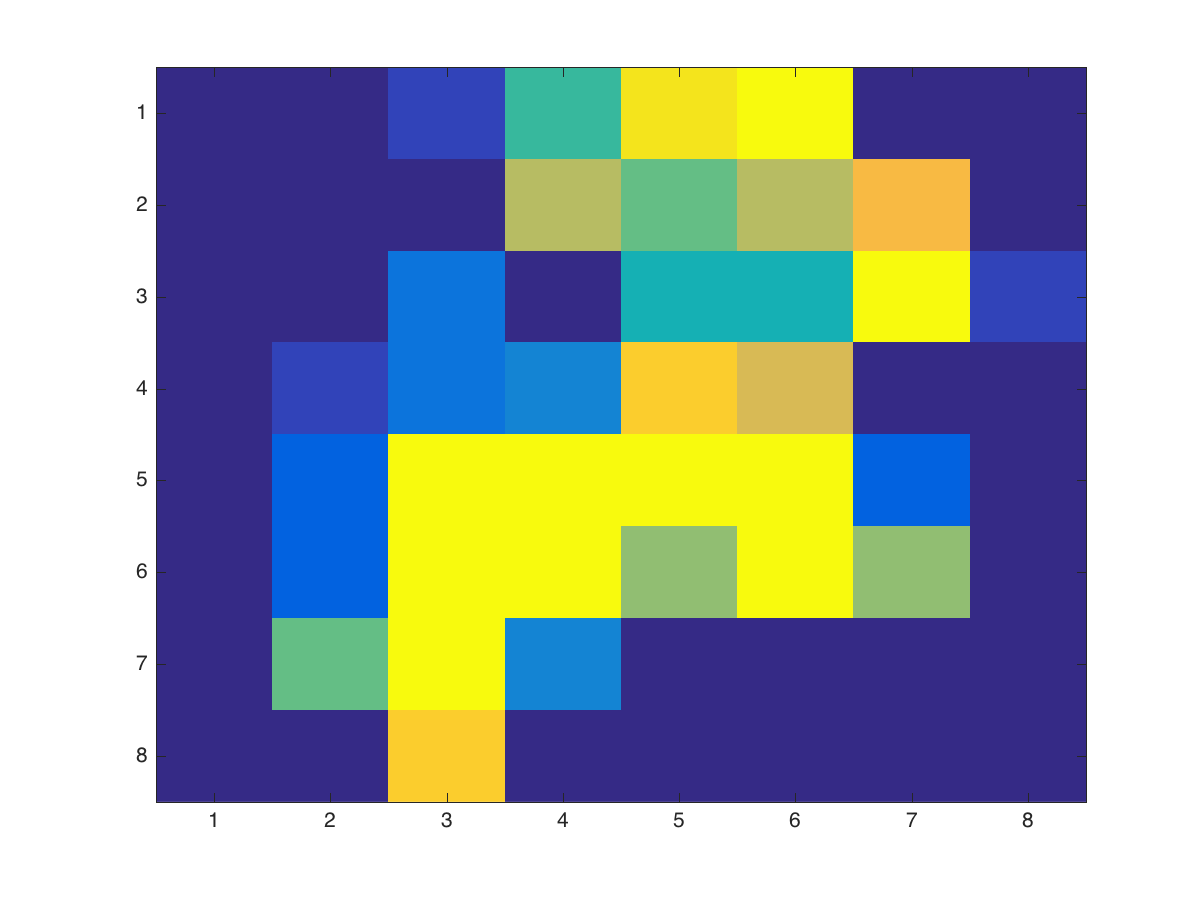
\includegraphics[width=0.4\textwidth]{seven_rotated.png}
\caption{Example images from training set}
\label{fig:rotated}
\end{figure}
\section{Design}

Network training is done off-line with a fixed batched size that is optimised experimentally. Batch training ensures a more smooth decent of the gradient error cost. Additionally a varying learning rate is used. This decreases in value with each complete iteration of the training set. The decay of the learning rate was also optimised experimentally. There is one single learning rate used for both the output layer and hidden layer.

Network training stops after a fixed number of epochs was trained. An epoch was considered as one single update of the weights. Although the network may stop at a point where the error cost is high, the approach avoid situations where the network would never complete training ( i.e. when choosing an error cost that can not be achieved). The optimal number of epochs was also discovered experimentally. 

Network training also employs a simple weight decay function ( i.e. decreasing the weights by a ratio of their current value). The decay ratio was optimised experimentally. 

\section{Implementation}

The neural network was implemented using matlab. Even though matlab has a specialised toolbox for neural networks, the project implements its own network and back-propagation algorithm. Matlab was chosen do to its inbuilt matrix operations, mathematical tools and visualisation features (e.g. error cost plotting). When adding image rotations to the training set, the image processing toolbox further simplified code complexity as algorithms were readily available.

\subsection{Initialisation}

The entry file to training a network is \emph{train.m}. At the start of execution the training set is loaded and extended with additional records for digit rotations (using \emph{addrotations.m}). The resulting training set is three times larger, having one clockwise and one counter clockwise rotation for each digit. The image processing toolbox from matlab was used to achieve this. Resulting records are then arbitrarily shuffled.

The  training set is further extended with additional features (i.e. covariance and mean pixel location). After extension, the features are normalised and scaled up ( i.e. by multiplying by a number larger than 1). The feature extension and normalisation represent a single step named preprocessing. It is handled by \emph{preprocess.m}.

The target class for the training set is separated from the features. Each target is transformed from a single digit to a 10 dimension vector. The vector represents the probability of each class occurring, meaning it has the value 1 on the class's position and 0 otherwise. 

\subsection{Training}

When training a network, it is first initialised with random weights drawn from a uniform distribution of $[-0.5,+0.5]$. The training is implented using vector and matrix multiplication instead of iterating through individual positions of weight updates. This method is called vectorisation and takes advantage of matlab's advanced optimisations in matrix operations, having faster training performance.

The output of the hidden layer is first calculated using the sigmoid activation function on an input batch. It then gets used as input in calculating the total network output using the softmax function. These are handled, in vector notation, by \emph{sigmoid.m} and \emph{softmax.m}.
\begin{lstlisting}
out{1} = [ones(size(batch,1),1) sigmoid(batch,w{1})];
out{2} = softmax(out{1},w{2});
\end{lstlisting}

The delta of each weight update is calculated using the first derivative of the cost function for each layer (following course formulas). The weight are updated by a proportion of the delta and also suffer a weight decay proportional to their current value. 

The bias unit is added to each layer input (i.e. training set input and hidden layer output). In calculating the weight delta, the value is removed whilst propagating errors back through the network. 

\subsection{Testing}

After training, the network weights are measured on the loaded test set. The set is processed similarly to the training one(i.e. through additional features and normalisation). When calculating the result of a given input, the predicted class is determined by selecting the output position with the highest probability value. Network performance is determined from the number of correctly predicted classes. 

\section{Experiments}

\subsection{Single Layer Experiments}
In order to establish a baseline of performance the network was initially built as a single layer perceptraon network with a fixed learning rate($\mu$), number of epochs and batch size. Each experiment trained and measured network performance 10 times for a better estimation of optimisation improvements. 

\subsubsection{Learning Rate}

For the initial training no preprocessing was done on the data set. Because of using the softmax activation function, a batch size larger than 20 or a learning rate larger than 0.01 could not be used as the the function would overflow double precision data types.

\begin{figure}
\centering
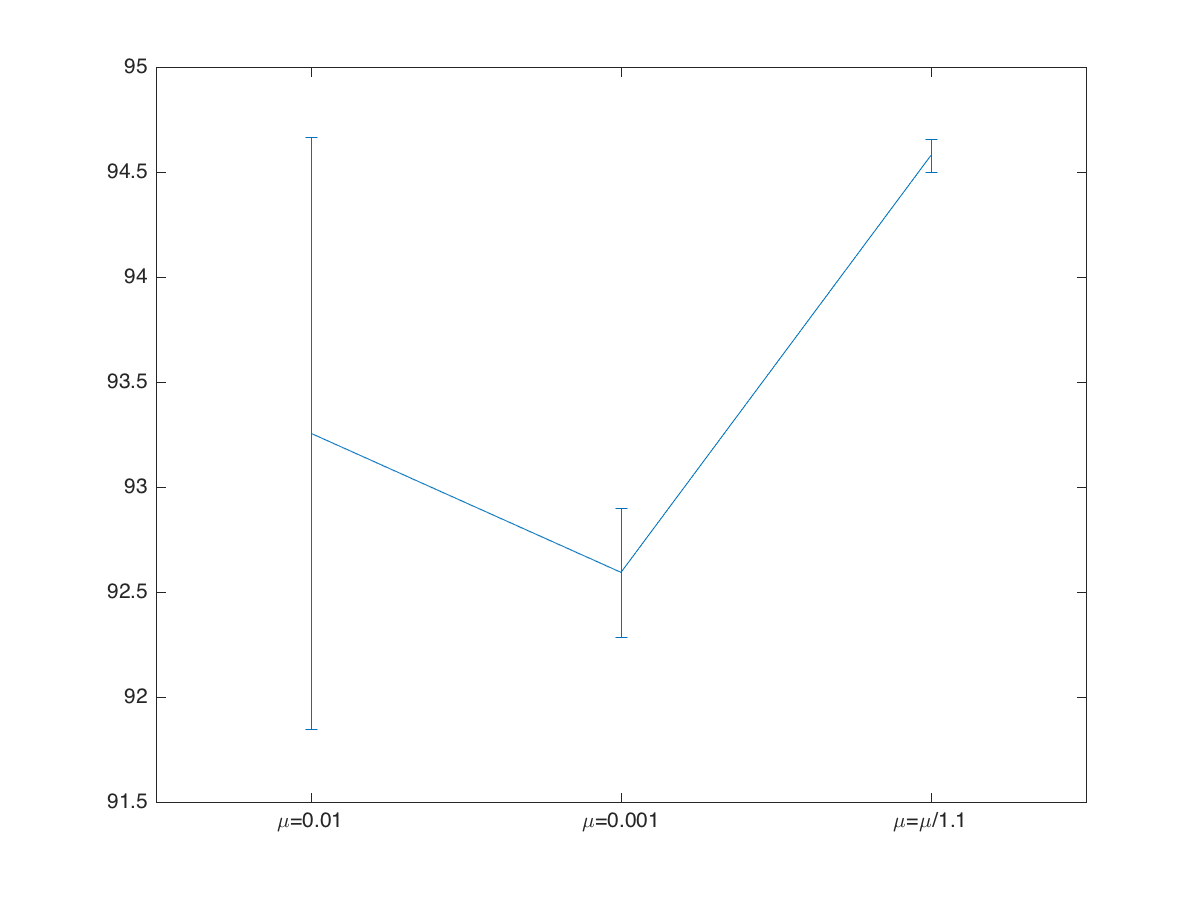
\includegraphics[width=0.9\textwidth]{learning_rate.png}
\caption{Adjusting learning rate $\mu$}
\label{fig:learningrate}
\end{figure}

With the initial batch=20, epoch=2000 and $\mu=0.01$, the network achieved an average 93.25\%($\pm 1.4\%)$ prediction success on the testing set.  A lower learning rate of $\mu=0.001$ was tried which produced a performance of 92.59\%($\pm 0.3\%$). Although average performance was lower in this case, the deviation in learning was greatly reduced. Using a variable learning rate the performance was further improved to 94.57\%($\pm 0.07\%$) signifying a great improvement in both performance and stability (fig. \ref{fig:learningrate}). The learning rate decay per each complete iteration of the training set is defined as $\mu = \mu / 1.1$ starting with $\mu=0.01$. Reducing the rate by larger or lower ratio would degrade performance. 

\subsubsection{Batch and Epoch Sizes}
Whilst a varying learning rate increase performance significantly, batch and epoch sizes were also experimented with (fig. \ref{fig:batchandepoch}). A low epoch size would underfit general training performance, whilst a low batch size would produce a less stable gradient descent. No further performance improvements were achieved when modifying these parameters. 

\begin{figure}
\centering
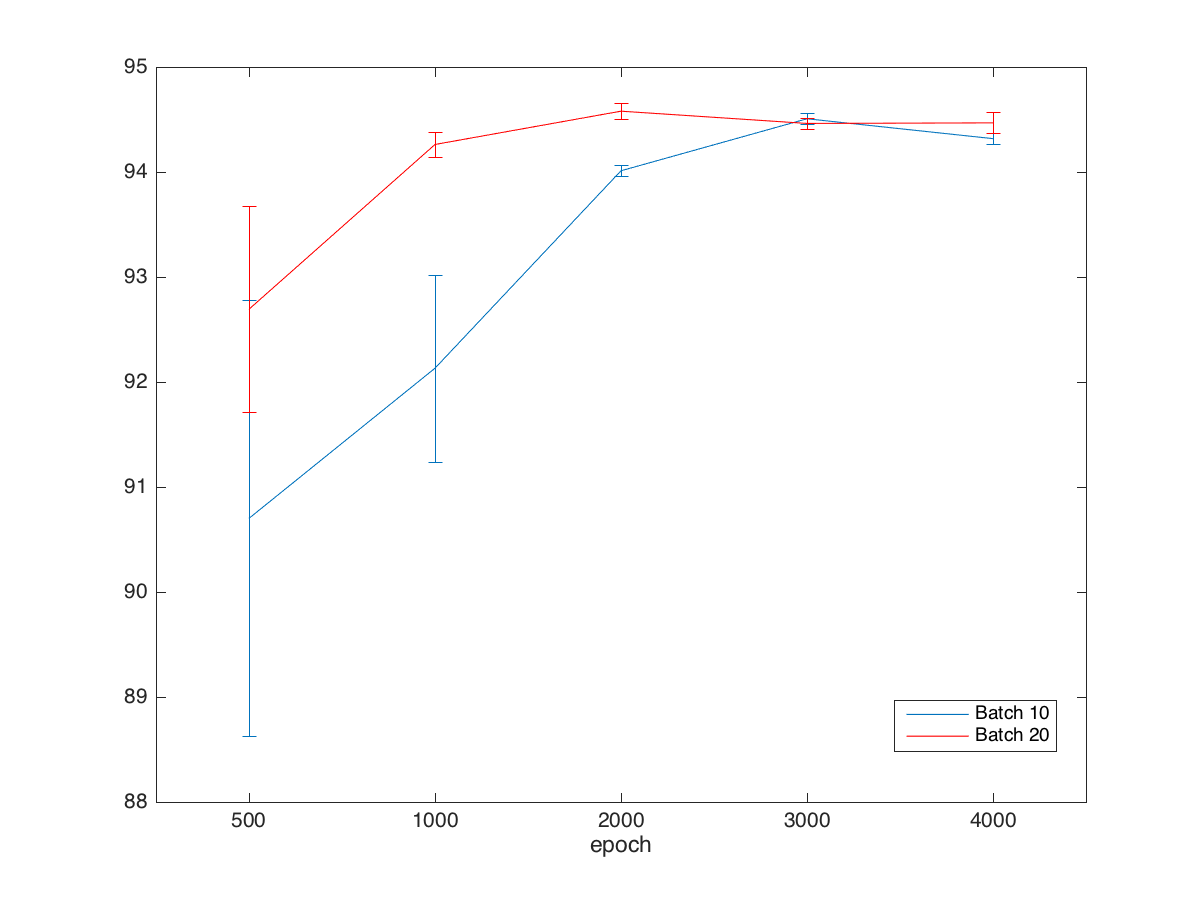
\includegraphics[width=0.9\textwidth]{batchandepoch.png}
\caption{Adjusting the batch and epoch sizes}
\label{fig:batchandepoch}
\end{figure}

\subsubsection{Preprocessing}
To further increase performance, preprocessing was done to both the training and test sets. As mentioned previously, additional features were generated based on existing features. All values were then normalised between $[0,12]$. Different scale intervals were tested although their results will not be mentioned. 

The technique improved average network performance to a mean of 95.11\%($\pm 0.01\%$) (fig. \ref{fig:normalised}). By normalising the data, the network could be trained with larger batch sizes and learning rates without number overflows. However, increasing these values did not further improve performance. 

\begin{figure}
\centering
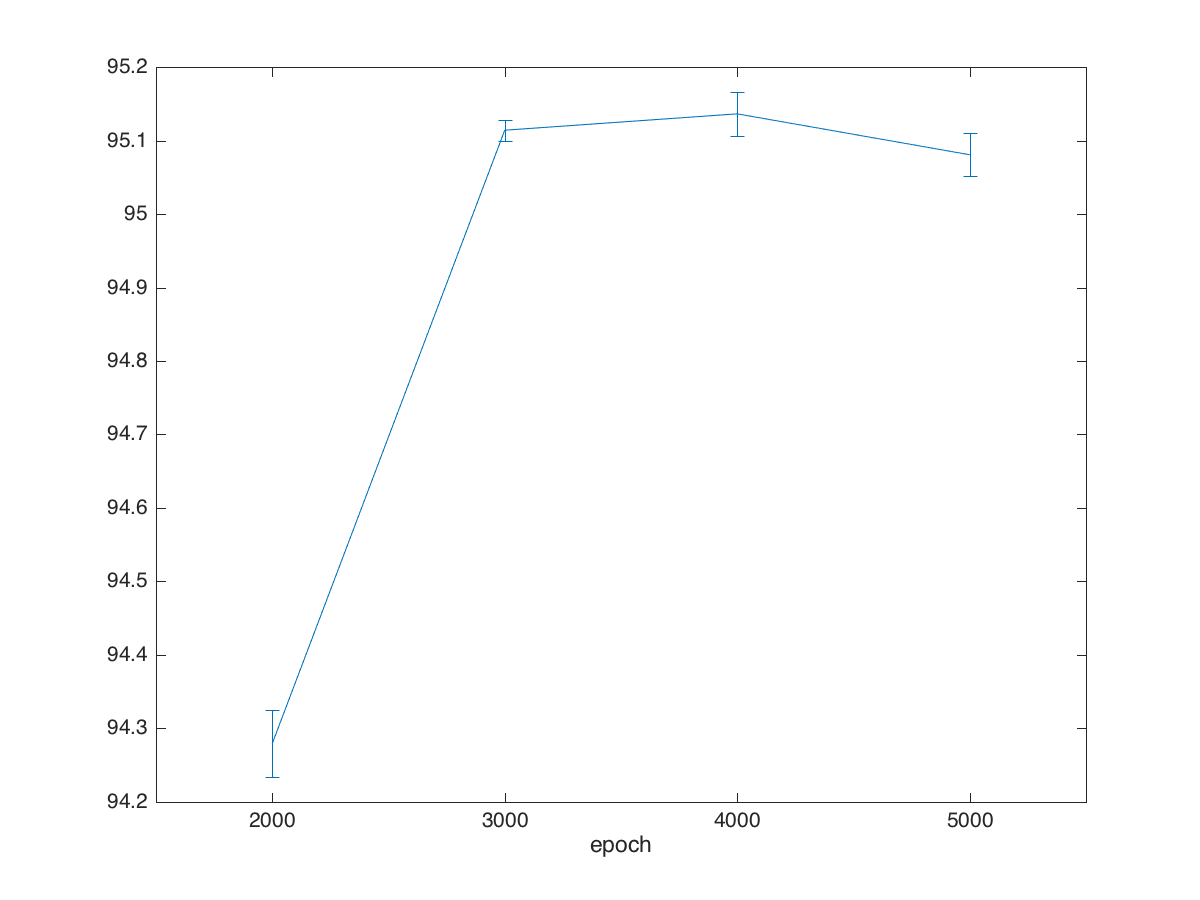
\includegraphics[width=0.9\textwidth]{normalised.png}
\caption{Preprocessing}
\label{fig:normalised}
\end{figure}

\subsection{Two Layer Experiments}

To understand what types of digits the network failed to predict, some of the test networks were viewed.  Most of the failings were rotated digits. Pixel covariance was meant to signal digit's rotation.  Covariance values are is analogous to orientation. Unfortunately, the approach was not sufficient. Either the covariance failed at indicating rotation, or the network did not have enough potential to generalise. 

\subsubsection{Hidden Unit Count}

An attempt at predicting rotated digits was to add a hidden layer to the network. The network could now be optimised in the number of hidden units. Other parameters of such as the batch size and epoch count required readjusting. The below graph (fig. \ref{fig:hiddenunits}) shows improved overall average performance for a batch size of 30 and epoch count of 5000.  Mean network performance in this case reached 96.2\%($\pm 0.1\%$) for a 90 units hidden layer. 
\begin{figure}
\centering
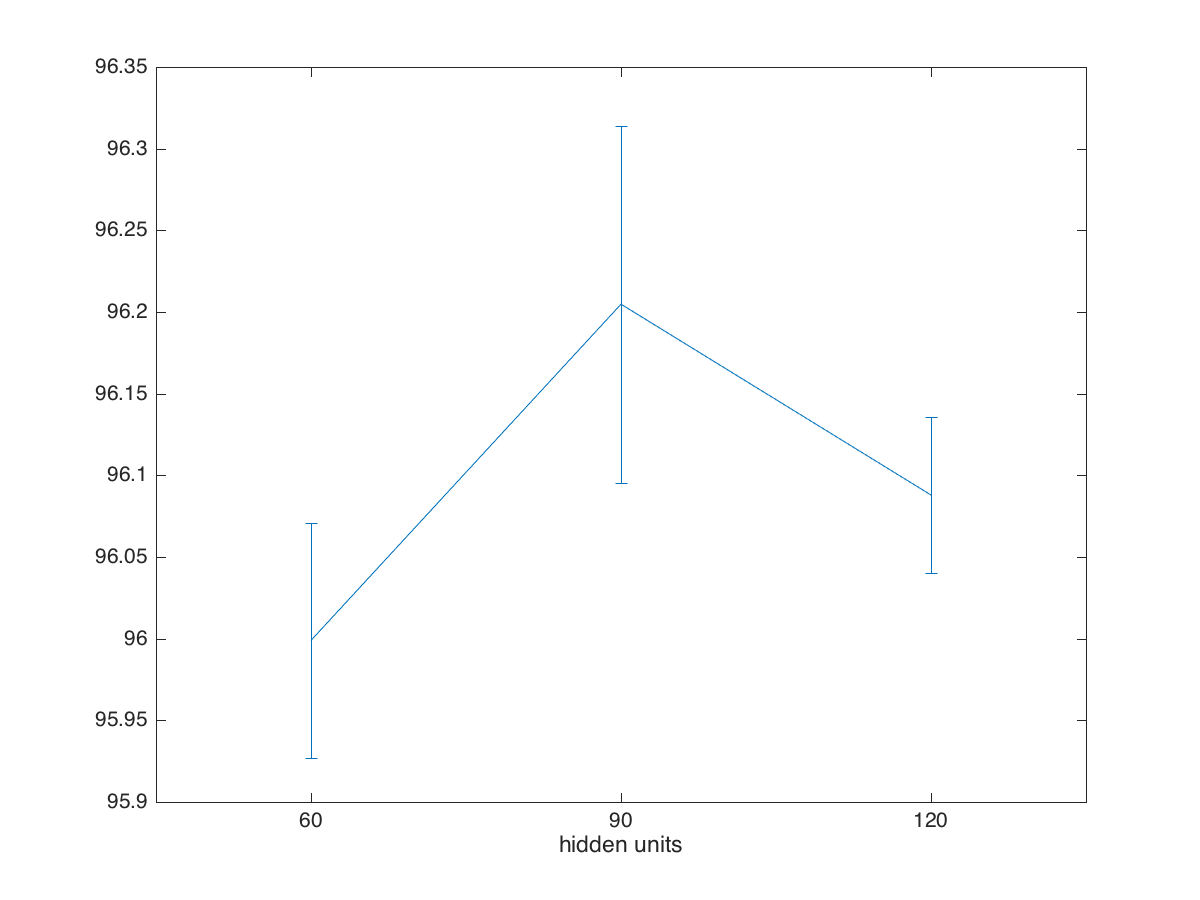
\includegraphics[width=0.9\textwidth]{hiddenunits.png}
\caption{Adjusting the number of hidden units}
\label{fig:hiddenunits}
\end{figure}

\subsubsection{Weight Decay}
A simple improvement that can raise generalisation is regularisation through weight decay. With this technique weights are constantly pushed towards a value of 0. The effect is of keeping weights inside a similar range of values. This prevents overshadowing of smaller weights by larger weights. In some sense it is similar to a form of normalisation.

Regularisation was implemented by adding or subtracting from a weight a ratio of its current value. Decay ratio can be seen as another parameter that can be optimised. Experimentally the best performance achieved with weight decay had a performance of 96.45\%($\pm 0.06\%$) (fig. \ref{fig:regularisation}).  Although the overall  improvement was not significant the change lead to a smaller standard deviation in training. All other parameters remained with previous values ( i.e. batch size 30, hidden units 90,epoch size 90, variable learning rate).

\begin{figure}
\centering
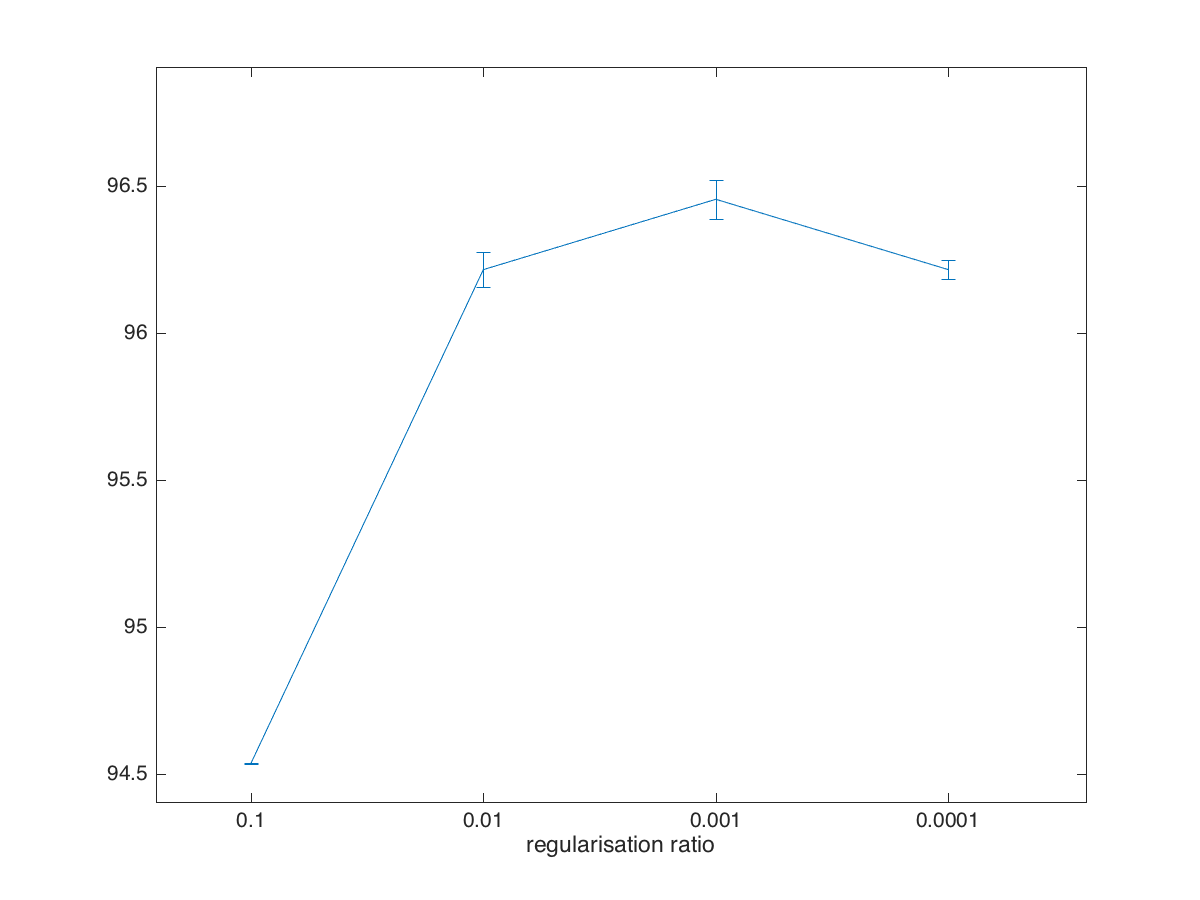
\includegraphics[width=0.9\textwidth]{regularisation.png}
\caption{Adjusting decay ratio}
\label{fig:regularisation}
\end{figure}

\subsection{Digit Rotations}
As most prediction failures in the testing set were rotated digits, it was necessary to create additional examples of rotations in order to further improve performance. Adding rotations tripled the training set and required adjusting the batch size, epoch count and number of hidden units. The below figure \ref{fig:rotations} demonstrates the effects of adjusting each such parameters. Even though prediction performance was higher, the optimising parameters became more difficult. 

\begin{figure}
\centering
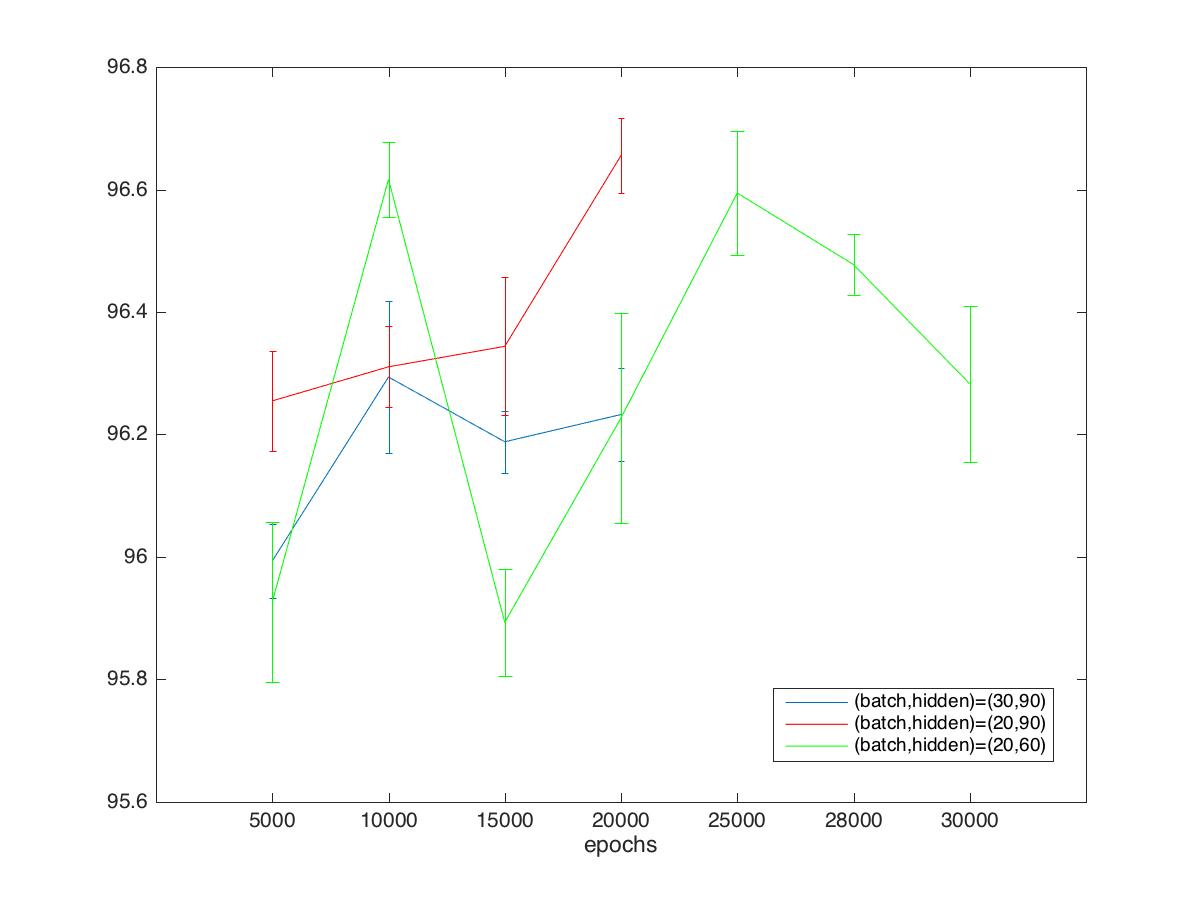
\includegraphics[width=0.9\textwidth]{rotations.png}
\caption{Adjusting parameters after rotation with decay 0.0001}
\label{fig:rotations}
\end{figure}

After increasing the weight decay ratio from 0.0001 to 0.001 performance slightly improved (fig. \ref{fig:rotations2}). The mean prediction achieved was 96.83\%($\pm 0.06\%$). A lack of predictability in optimisations may be due to the training set being randomly expanded with rotations. Variability in training data may therefore affect prediction performance. Rotations are not reset after each network training, so even though 10 networks are trained they are all likely to optimise for a training set that is less compatible with the test set. 

However, through this method the best achieved performance was 97.21\%. The best obtained weights can be loaded and tested against the training set by running \emph{showdigits.m}. The script also shows the digits that failed recognition. 

\begin{figure}
\centering
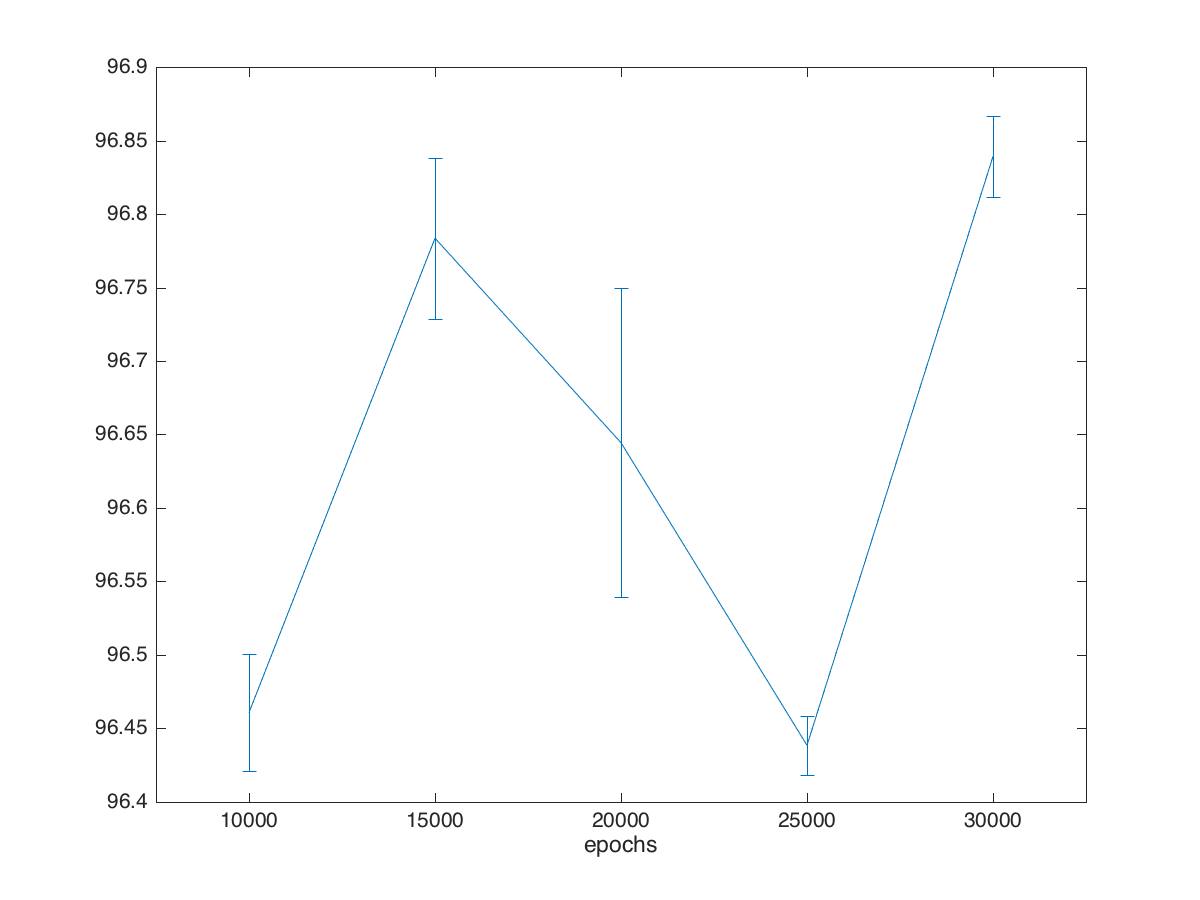
\includegraphics[width=0.9\textwidth]{rotations2.png}
\caption{Adjusting decay 0.001, batch size 20 , hidden 90}
\label{fig:rotations2}
\end{figure}

\section{Conclusions}
Surprisingly, a single layer network was able to achieve a significantly high generalisation of 92.5\% prediction performance. The most important improvement was  gained from implementing a variable learning rate. Whilst performance increased (by 2\% to a total of 94.5\%), the standard deviation also decreased from 0.3\% to 0.07\%.

The next most significant improvement was adding a hidden layer to the network. The average performance improved by another 1\% at the cost of a small increase in standard deviation (to 0.1\%).

With most implementation and design changes, the epoch and batch size had to be readjusted. This was especially true after adding input normalisation and input rotation. Altough improvements were not significant, these changes helped break the performance barrier to an ever high of 97.27\%. Variably rotating training data in order to create additional sets proved to make optimisation more difficult. 

\end{document}